% Figures/semicontinuity.tex
% Illustrates Definition \ref{def:semicontinuity} of Chapter \ref{ch:continuity}:
% at a point of upper semicontinuity the value sits at the top of a jump, at a
% point of lower semicontinuity at the bottom. Both panels show a function equal
% to a on one side of x_0 and to b > a on the other; only the value taken at
% x_0 itself differs.
% Source: Fukuda (2026), Supplementary Prop. 8.10 (p. 271).
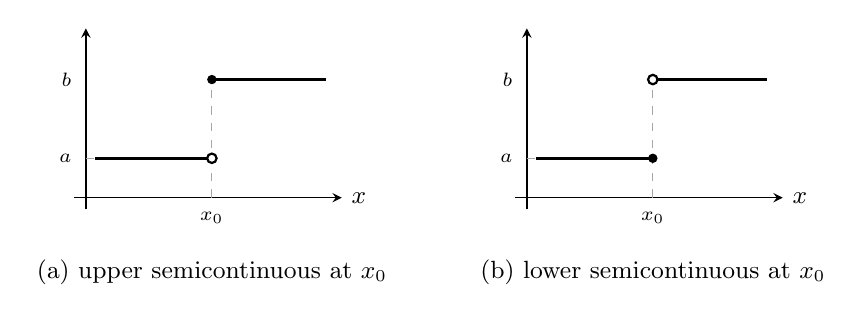
\begin{tikzpicture}[
		scale=1.0,
		>=stealth,
		curve/.style={line width=1.2pt},
		guide/.style={line width=0.4pt, black!35, dashed},
		panel/.style={font=\small},
	]

	% ---------- panel (a): upper semicontinuous ----------
	\begin{scope}
		\draw[->,line width=0.5pt] (-0.15,0) -- (3.25,0) node[right,font=\small] {$x$};
		\draw[->,line width=0.5pt] (0,-0.15) -- (0,2.15);
		\draw[guide] (1.6,0) -- (1.6,1.5);
		\draw[guide] (0,0.5) -- (1.6,0.5);
		\node[font=\scriptsize,anchor=north] at (1.6,-0.06) {$x_0$};
		\node[font=\scriptsize,anchor=east] at (-0.06,0.5) {$a$};
		\node[font=\scriptsize,anchor=east] at (-0.06,1.5) {$b$};
		\draw[curve] (0.12,0.5) -- (1.6,0.5);
		\draw[curve] (1.6,1.5) -- (3.05,1.5);
		\fill (1.6,1.5) circle (1.7pt);
		\draw[line width=0.8pt,fill=white] (1.6,0.5) circle (1.7pt);
		\node[panel,align=center] at (1.6,-0.95)
		{(a) upper semicontinuous at $x_0$};
	\end{scope}

	% ---------- panel (b): lower semicontinuous ----------
	\begin{scope}[shift={(5.6,0)}]
		\draw[->,line width=0.5pt] (-0.15,0) -- (3.25,0) node[right,font=\small] {$x$};
		\draw[->,line width=0.5pt] (0,-0.15) -- (0,2.15);
		\draw[guide] (1.6,0) -- (1.6,1.5);
		\draw[guide] (0,0.5) -- (1.6,0.5);
		\node[font=\scriptsize,anchor=north] at (1.6,-0.06) {$x_0$};
		\node[font=\scriptsize,anchor=east] at (-0.06,0.5) {$a$};
		\node[font=\scriptsize,anchor=east] at (-0.06,1.5) {$b$};
		\draw[curve] (0.12,0.5) -- (1.6,0.5);
		\draw[curve] (1.6,1.5) -- (3.05,1.5);
		\fill (1.6,0.5) circle (1.7pt);
		\draw[line width=0.8pt,fill=white] (1.6,1.5) circle (1.7pt);
		\node[panel,align=center] at (1.6,-0.95)
		{(b) lower semicontinuous at $x_0$};
	\end{scope}

\end{tikzpicture}
